\documentclass[12pt]{article}
\usepackage[a4paper, total={6in, 9in}]{geometry}
\usepackage{amsmath, amssymb}
\usepackage{graphicx}
\usepackage{enumitem}
\usepackage{fancyvrb}
\usepackage[skip=\medskipamount]{parskip}
\usepackage{pdfpages}
\usepackage{array}
\usepackage{tabularray}
\usepackage{longtable}
\usepackage{tikz}
\usepackage{float}
\setlength{\parindent}{0pt}

% \renewcommand*{\thesubsection}{\alph{subsection}}
% \renewcommand*{\theenumi}{\alph{enumi}}

\title{\vspace{-1.5cm}E0 259 Assignment-4}
\author{Aditya Gupta \\
SR No: 22205}
\date{}

\begin{document}
\maketitle

\section*{Implementation Summary}
We have to implement the Duckworth Lewis method for estimation of target score in a rain affected match. We have data corresponding to several one day matches given to us. We will use this to estimate the set of constants for the Duckworth Lewis method formula, which is given by:
\begin{equation*}
    Z(u, w) = Z_0(w)[1 - e^{-Lu/Z_0(w)}]
\end{equation*}
where $Z(u, w)$ is the target score, $u$ is the number of overs remaining to be bowled, $w$ is the number of wickets in hand and $Z_0(w)$ is the series of constants.

First, we solve this by replacing $L$ with $L(w)$, where $L(w)$ is a linear function of $w$. Thus we need to find the value of 20 constants, $Z_0(w)$ and $L(w)$ for $w = 1, 2, \ldots, 10$.
\begin{equation*}
    Z(u, w) = Z_0(w)[1 - e^{-L(w)u/Z_0(w)}]
\end{equation*}

We know the actual score of each match from the data provided to us. First, we perform some preprocessing on the data given to us. The data provided has the information of the team's total score and wickets in hand at the end of each over and the final score they ended up with. If we are given the score at the end of the $i^{th}$ over with $j$ wickets in hand, then we have that:
\begin{equation*}
    Z(50 - i, j) = \text{final score} - \text{score at the end of the } i^{th} \text{ over} 
\end{equation*}

We get this information for each datapoint given to us and use it as the actual score for the Duckworth Lewis method. Now we can predict the score and use a loss function to calculate the error and optimise it. The loss function used is:
\begin{equation*}
    loss(y', y) = (y' + 1) \log((y' + 1)/(y + 1)) - (y' - y)
\end{equation*}
where $y'$ is the predicted score and $y$ is the actual score. We use this loss function to calculate the error and optimise using the Limited Memory BFGS method provided by the scipy library.

Once we calculate the optimal values of $Z_0(w)$ and $L(w)$, we use a weighted average of the values of $L(w)$ to get the final value of $L$, where the weights of $L(w)$ are given by the number of datapoints with $w$ wickets in hand. Using this value of $L$, we once again run the same optimisation process to get the final values of $Z_0(w)$.

Finally we store the model weights and plot the graphs of the Duckworth Lewis functions for each set of weights. We also calculate the normalised mean squared error for the final model.


\section*{Results}
\subsection*{Initial Weights}
The initial 20 weights for the model are:
\begin{align*}
    &Z_0[1]: 6.604864967654443    &&L[1]: 6.37539793757683 \\
    &Z_0[2]: 19.52808599501093    &&L[2]: 7.995440493101641 \\
    &Z_0[3]: 40.514984506310704   &&L[3]: 10.403271144445565 \\
    &Z_0[4]: 66.72055933509327    &&L[4]: 10.265091187424519 \\
    &Z_0[5]: 91.36895005148128    &&L[5]: 10.539957611689532 \\
    &Z_0[6]: 122.32217000616183   &&L[6]: 11.19657221841599 \\
    &Z_0[7]: 157.89111447218542   &&L[7]: 10.691521698958688 \\
    &Z_0[8]: 196.9245538104981    &&L[8]: 10.638527672168712 \\ 
    &Z_0[9]: 220.99159594799406   &&L[9]: 11.287089464581245 \\
    &Z_0[10]: 258.52854290234336  &&L[10]: 11.652052372738092 
\end{align*}

The log loss associated with this set of weights is 6.410156648717406

\begin{figure}[H]
    \centering
    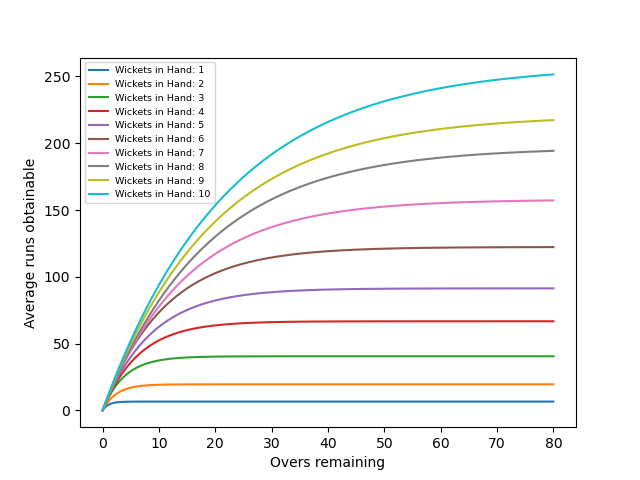
\includegraphics[width=\textwidth]{plots/22205_Plot1.png}
    \caption{Duckworth Lewis functions for initial weights}
\end{figure}

\subsection*{Final Weights}
The final 11 weights for the model are:
\begin{align*}
    &Z_0[1]: 6.242999827362688 \\
    &Z_0[2]: 18.796065534214872 \\
    &Z_0[3]: 39.99808134110431 \\
    &Z_0[4]: 65.79769756300017 \\
    &Z_0[5]: 91.01238598239004 \\ 
    &Z_0[6]: 124.61817051017574 \\
    &Z_0[7]: 156.42387207633024 \\
    &Z_0[8]: 194.5808563258143 \\
    &Z_0[9]: 225.7662005766769 \\
    &Z_0[10]: 269.5264558576793 \\
    &L: 10.79572686731456
\end{align*}

The log loss associated with this set of weights is 6.415204555413272

The normalised mean squared error (sum of square of differences, divided by the total no. of datapoints) for this set of weights is 1678.6395442700937

\vspace*{-1mm}
\begin{figure}[H]
    \centering
    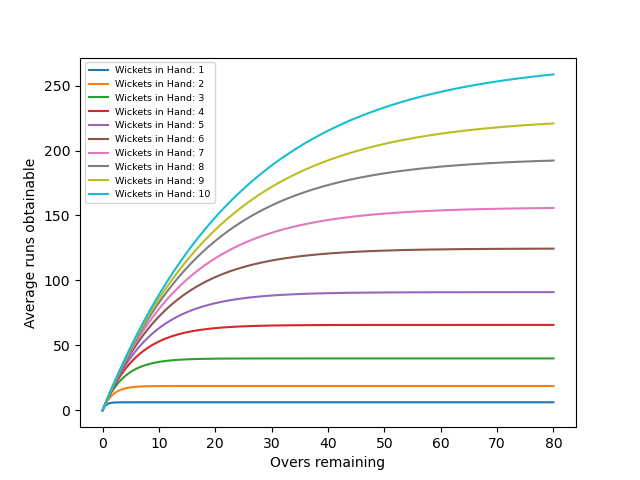
\includegraphics[width=\textwidth]{plots/22205_Plot2.png}
    \caption{Duckworth Lewis functions for final weights}
\end{figure}

\end{document}